%  LP: la partie commentee ci-dessous a ete copié dans le fichierA
%  ``reference_flux.tex'' (peut etre supprimee ici)

%\subsubsection{Reference flux densities of secondary calibrators}
%\label{se:fluxSec}
%(revised by JFL Aug 2017 - must remove the old version in photometry-HA.tex)
%

%++ SPIRE refer.


%% Shortened version by LP, the original version can be found in the appendices


\section{Flux density stability with aperture photometry {\color{green} Jean-Fran\c cois}}
\label{se:aperture_photometry}

%As a consistency check of the baseline calibration results that rely on PSF fitting, we have also used aperture photometry to recover as much as possible of the calibrator flux spread over the main beam and side
%lobes of the telescope when assessing the stability of the
%calibration.
 
Aperture photometry was used to measure the flux densities of  primary calibrators Uranus and Neptune
and  secondary calibrators MWC349A, NGC7027 and CRL2688.   These
sources are point-like, except Uranus and Neptune that are small disks
($\sim 3.5''$ and $\sim 2.5''$ in diameter, respectively), and NGC7027 which is somewhat
extended ($\sim 10''$).

We have implemented aperture photometry as described in
\S~\ref{se:aperture_photo_calibration} with the constant solid
angles $\Omega_{tot}$ given in Table ~\ref{tab:solid} for each array (mean), and the
NIKA2 gain-elevation curve of the Pipeline. The aperture radius was
$150''$ and suitable for all calibrators except for MWC349A
whose flux densities became somewhat unstable over such a large
aperture. For this source, we reduce the aperture to $60''$ but
corrected the resulting flux densities by factor 1.08 for arrays A1
and A3, and factor 1.05 for array A2. These factors were derived from the very clean integrated flux
curves obtained with the Uranus observations 20170227s308 (see Figure \ref{fig:Uranus_s308}).  
Color-corrections from Table~\ref{tab:mod}   have been applied
with indices $\alpha=+0.6$, $-0.34$ and $+2.44$ for MWC349A, NGC7027
and CRL2688, respectively.

Measured flux densities are reported in Table~\ref{tab:flux_Ap}
and the  stability for these calibrators  are shown in Figure~\ref{fig:stab}. We conclude that :




\begin{table}[th]
\begin{center}
\begin{threeparttable}
\begin{tabular}{|c|c|c|c|c|c|}
\hline
\multicolumn{3}{|c}{}  & \multicolumn{3}{|c|}{Flux densities (Jy)}   \\
\hline
         & run  & \#obs &  A1                    &  A2                   &    A3                    \\
         &      &      &  $S_{260 {\rm GHz}}$     &  $S_{150 {\rm GHz}}$  & $S_{260 {\rm GHz}}$    \\
\hline\hline
MWC349A   &  9   & 61  &  $2.10\pm0.03$   &  $1.41\pm0.005$  &  $2.07\pm0.03$       \\
  $''$    & 12   & 11  &  $2.38\pm0.1$   &   $1.40\pm0.016$ &  $2.06\pm0.08$                  \\ 
  $''$    & 14   & 32  &  $2.22\pm0.04$   &  $1.42\pm0.009$ &  $2.20\pm0.05$                  \\
  \hline
NGC7027  &  9   & 75  &  $4.58\pm0.05$   &  $4.52\pm0.01$  & $4.66\pm0.04$        \\
  $''$   & 12   &  3  &  $4.65\pm0.28$   &  $4.67\pm0.1$  & $4.82\pm0.30$                    \\ 
  $''$   & 14   &  0  &    -             &  -              &  -                   \\
  \hline
CRL2688  &  9   & 68  &  $2.81\pm0.03$   &  $0.55\pm0.003$   &  $2.83\pm0.03$      \\
  $''$   & 12   &  5  &  $2.85\pm0.16$   &  $0.54\pm0.02$    &  $3.01\pm0.19$                   \\
  $''$   & 14   &  3  &  $2.98\pm0.10$   &  $0.57\pm0.006$   &  $3.06\pm0.21$                   \\
\hline
\end{tabular}
\begin{tablenotes}
{\small
  \item[]  Uncertainties are statistical only ($rms/\sqrt{\#obs}$).
}
  \end{tablenotes}
\end{threeparttable}
\caption{Flux densities from aperture photometry.}
\label{tab:flux_Ap}
\end{center}
\end{table}


\begin{figure}[ht!]
  \begin{center}
    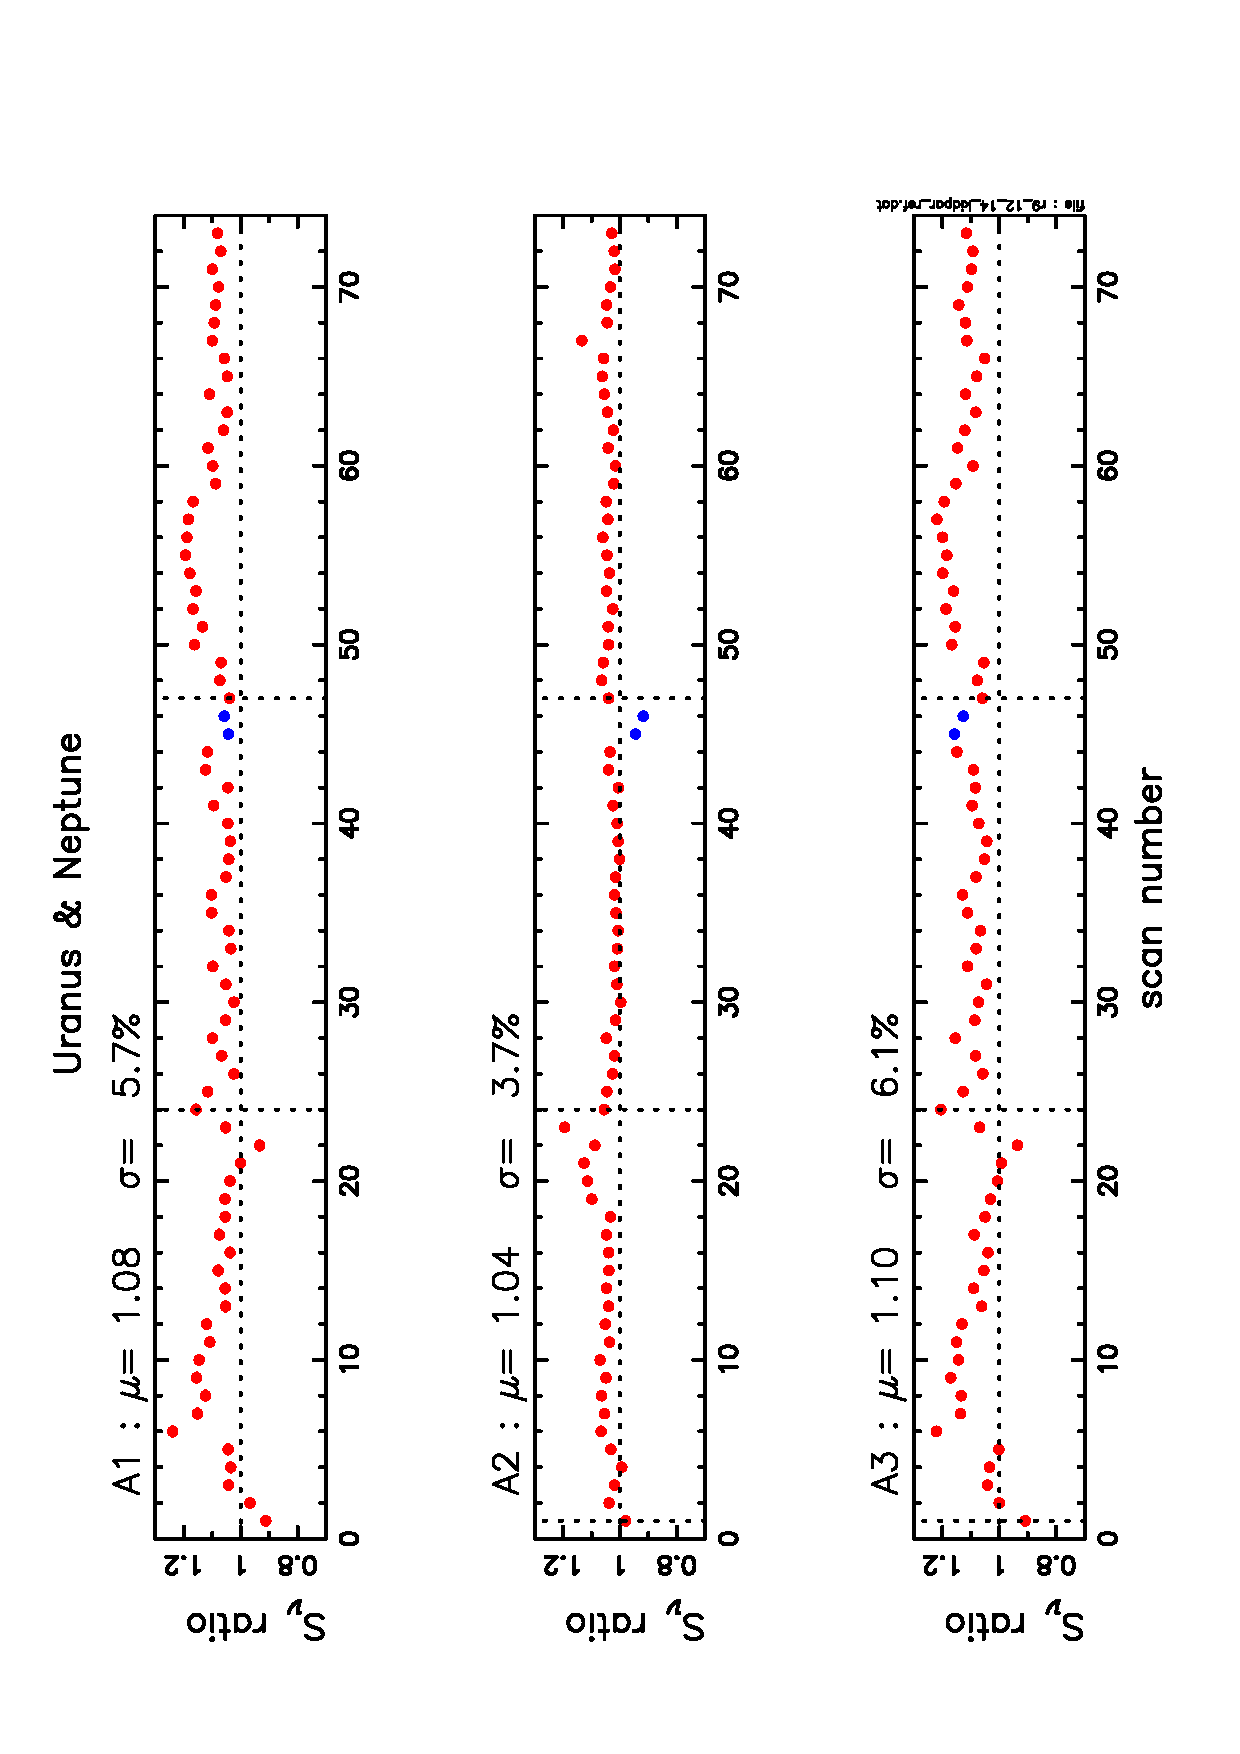
\includegraphics[clip=true,angle=-90.,width=0.55\textwidth]{Figures/Aperture_photo/Ura_Nept_Flux_ratio_index_A1_A2_A3.pdf},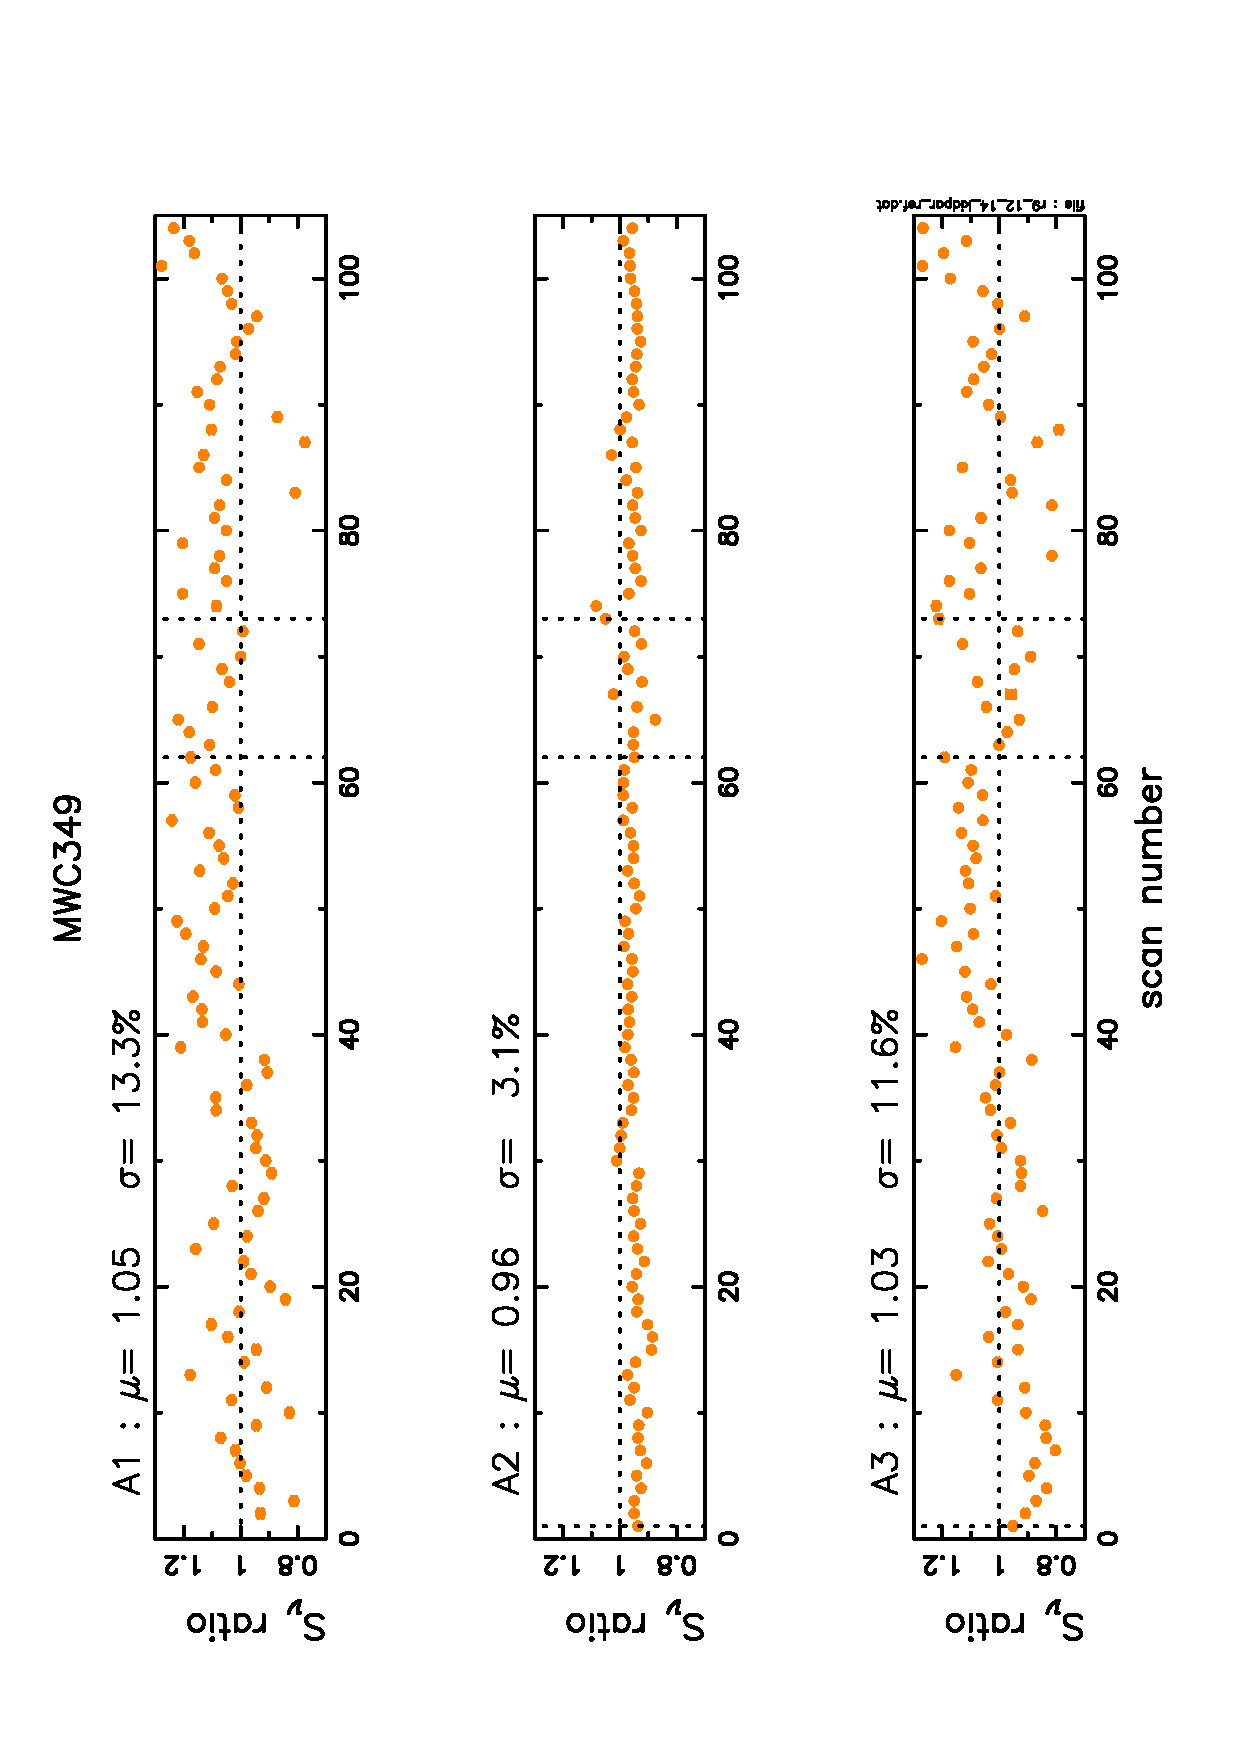
\includegraphics[clip=true,angle=-90.,width=0.55\textwidth]{Figures/Aperture_photo/MWC349_Flux_ratio_index_A1_A2_A3.pdf}
    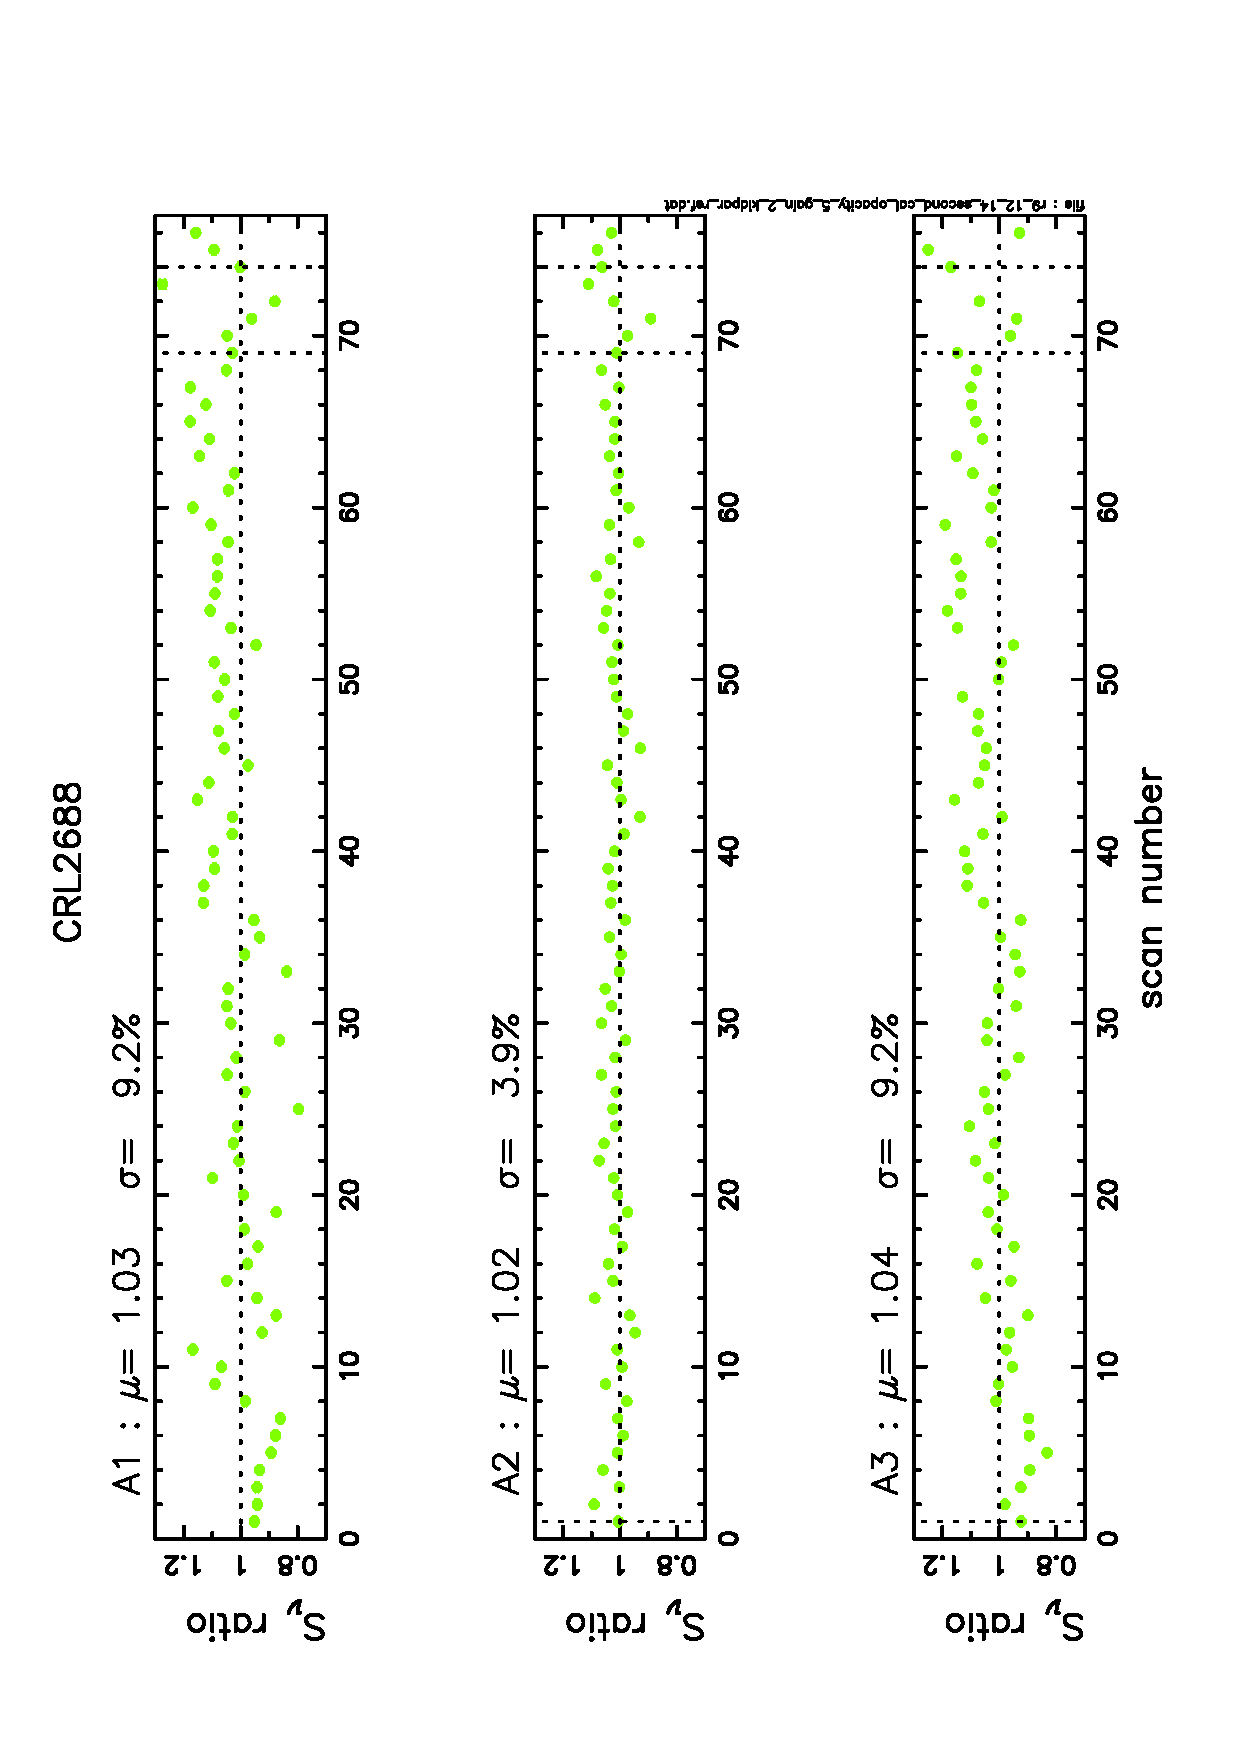
\includegraphics[clip=true,angle=-90.,width=0.55\textwidth]{Figures/Aperture_photo/CRL2688_Flux_ratio_index_A1_A2_A3.pdf},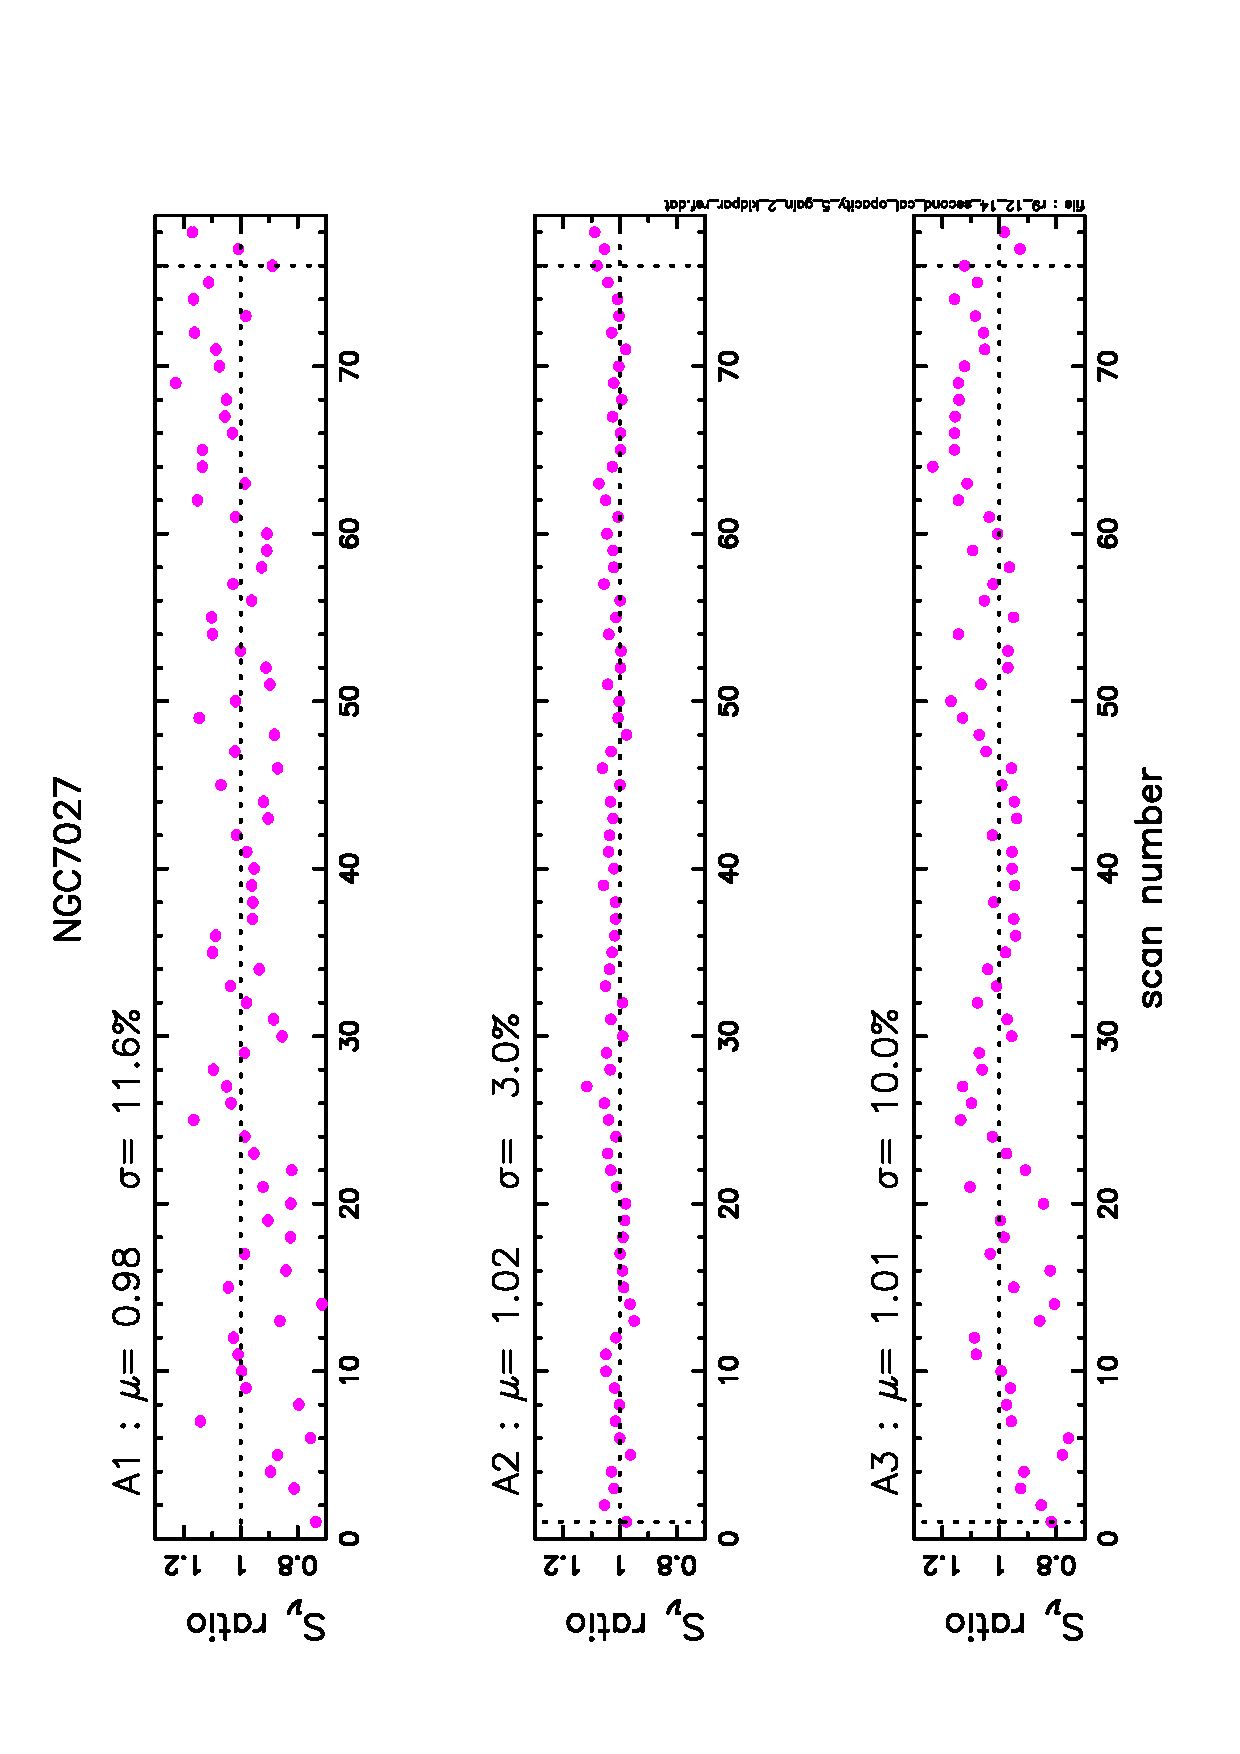
\includegraphics[clip=true,angle=-90.,width=0.55\textwidth]{Figures/Aperture_photo/NGC7027_Flux_ratio_index_A1_A2_A3.pdf}
    \caption{Stability of primary and secondary flux density calibrators in runs 9, 12 and 14 displayed sequentially and separated by vertical dotted lines. Top-left : Aperture photometry of Uranus (red) and Neptune (blue). Flux ratios with respect to
reference flux densities from planet atmospheric models at 260 and 150 GHz adopted to establish the  reference kidpars.  
 Top-right~:~Aperture photometry of MWC349A. Bottom-left~:~CRL2688. Bottom-right~:~NGC7027 (no
 observations in run 14).     
Mean biases ($\mu$) and scatters ($\sigma$) are given.}
    \label{fig:stab}
  \end{center}
\end{figure}


\begin{itemize}
  
\item measured flux densities of Uranus and Neptune are 5-10\% higher than the  values expected from the atmospheric models of these 
planets in Table~\ref{tab:fluxPred}. This apparent inconsistency can be explained by the fact that the flux density scale is given 
by gaussian fits of standard fwhms ($12.5''$ and $18''$) for Uranus when establishing the kidpars while the measurement in this section is based on aperture photometry. 
This ratio between aperture photometry and gaussian photometry has already been discussed in \S\ref{se:aperture_photo_calibration} (Table~\ref{tab:ratio}).


\item   measured flux densities of MWC349, NGC7027 and CRL2688 are consistent with expected values in Table~\ref{tab:flux_ref_sec} within uncertainties, 
except for NGC7027 which is 35\% higher than in this Table at 1mm, i.e. it is measured to be $4.7 \pm 0.2$ Jy while expected to be 
$3.46 \pm 0.11$ Jy. Confirmation of this flux density at 1mm 
 in the future  with NIKA2 should  lead to a revision of the SED of this source. Nonetheless, it remains that based on our comment above concerning
Uranus and Neptune,  flux densities of the three seconadry calibrators should have been biased upward by 5-10\% with aperture photometry also.
Consistency between  kidpar and aperture photometry remains an issue.    


\item discontinuties seen in photometry of Figures~\ref{fig:stab} are highly correlated with discontinuties in the opacity
when atmospheric conditions change and derived from the NIKA2 data themselves. This derivation might be improved in the future. 



\end{itemize}

























